\documentclass[11pt]{jarticle}
%
\usepackage[dvipdfmx]{graphicx}
\usepackage{amsmath}
\usepackage{amssymb}
\usepackage{bm}
\usepackage{latexsym}
\usepackage{float}
\usepackage{hyperref}
\usepackage[justification=centering]{caption}
%
\addtolength{\textwidth}{40mm}
\addtolength{\oddsidemargin}{-20mm}
\addtolength{\evensidemargin}{-20mm}
\addtolength{\textheight}{15mm}
\addtolength{\topmargin}{-10mm}
%
\pagestyle{empty}
%
\title{研究進捗報告}
\author{里谷 佳紀}
%\date{\today}
\date{平成29年9月25日}
%
\begin{document}
%
\maketitle
\thispagestyle{empty}
%
\section{研究全体の目標}
与えられた頂点数と次数をもつ正則グラフのうち,Cerfらの平均頂点間距離の下界\cite{Cerf1974}と一致する
平均頂点間距離をもつグラフが存在するかを判定する方法を開発する.
また,既存の方法\cite{Yamamoto2016}と比較することにより,新方法の有用性を検証する.

\section{前回打ち合わせ時に定めた短期目標}
\begin{enumerate}
\item 深さ優先探索によるグラフの発見
\item 命題
  \begin{enumerate}
  \item グラフ$G$に長さ$2Q$以下の閉路が存在せず,直径が$Q+1$ならば,
    $G$はCerfらの下界を達成する.
  \item \label{cycle-diam}
    グラフ$G$に長さ$2Q$以下の閉路が存在しないならば,直径が$Q+1$である.
  \end{enumerate}
  の検証
\end{enumerate}

\section{本日までの進捗状況}
\begin{enumerate}
\item プログラムが完成した.\\
  \url{https://gist.github.com/arity-r/21ded374488645fec6c3d1de9e6d3a83}(Python)と\\
  \url{https://github.com/y-satotani/cerfcheck}(C言語)にて公開している.
  さらに,いくつかの頂点数と次数の組み合わせで実験を行った.結果を表\ref{tab:result}
  に示す.
\item 命題\ref{cycle-diam}が偽になるグラフを発見した.図\ref{fig:cycle-diam}
  に示す.頂点数が14で,次数が3であるこのグラフは,
  最小の閉路長が5($>2Q$)であるが,直径は4($\neq Q+1$)である.
  さらに,このグラフはCerfらの下界を満足しない.
\end{enumerate}

\begin{table}[H]
  \centering
  \caption{実験結果 \\ 横に並んだ数字は頂点数を,縦に並んだ数字は次数を表す.
    \checkmark はプログラムが最初に発見したグラフがCerfらの下界を達成する
    組み合わせを,NAは正則グラフが存在しない組み合わせを表す.}
  \begin{tabular}{|c|c|c|c|c|c|c|c|c|c|}
    \hline
    & 4 & 5 & 6 & 7 & 8 & 9 & 10 & 11 & 12 \\ \hline
    3 & \checkmark & NA & \checkmark & NA & \checkmark & NA & \checkmark & NA & \checkmark \\ \hline
    4 & NA & \checkmark & \checkmark & \checkmark & \checkmark & \checkmark & \checkmark & \checkmark & \checkmark \\ \hline
    5 & NA & NA & \checkmark & NA & \checkmark & NA & \checkmark & NA & \checkmark \\ \hline
  \end{tabular}
  \label{tab:result}
\end{table}


\begin{figure}[H]
  \centering
  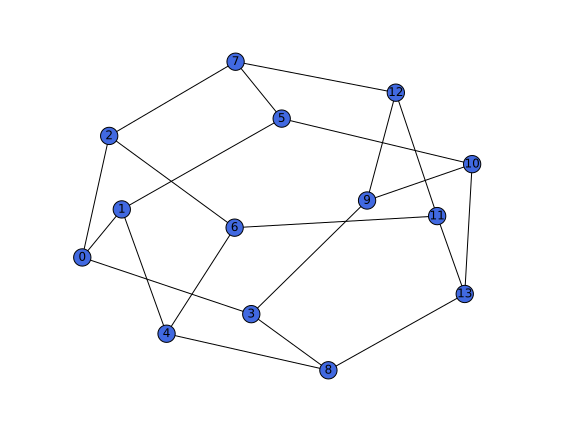
\includegraphics[width=\textwidth]{week2-graph.pdf}
  \caption{命題\ref{cycle-diam}の反例}
  \label{fig:cycle-diam}
\end{figure}

\bibliographystyle{junsrt}
\bibliography{refs}

\end{document}
